\subsubsection*{6.}
PWMの周波数が十分高いとき,微小時間で平均すると各相の波形は正弦波になる.すなわち各相の波形は
\begin{align*}
  v_{uo}&\propto \sin\omega t\\
  v_{vo}&\propto \sin\left(\omega t+\frac{2\pi}{3}\right)\\
  v_{wo}&\propto \sin\left(\omega t+\frac{4\pi}{3}\right)
\end{align*}
である.中性点の電圧は
\begin{align*}
  v_{no}=v_{uo}+v_{vo}+v_{wo}
\end{align*}
である.これは単位円を用いて考えることができる.これらは図\ref{fig:circle}の各点の虚部に当たるが,
正三角形の重心の公式から
\begin{align*}
  z_G=0=\frac{z_A+z_B+z_C}{3}
\end{align*}
である.したがって
\begin{align*}
  v_{no}=0
\end{align*}
となる.以上から中性点に流れ込む電力は
\begin{align*}
  P&\propto v_{uo}^2+v_{vo}^2+v_{wo}^2\\
  &=\sin^2\omega t+\sin^2\left(\omega t+\frac{2\pi}{3}\right)+\sin^2\left(\omega t+\frac{4\pi}{3}\right)\\
  &=\frac{1}{2}\left(1-\cos2\omega t+1-\cos\left(2\omega t+\frac{4\pi}{3}\right)+1-\cos\left(2\omega t+\frac{8\pi}{3}\right)\right)\\
  &=\frac{3}{2}
\end{align*}
となり定数になる.以上から入力電力は一定になる.
\begin{figure}[htbp]
  \begin{center}
    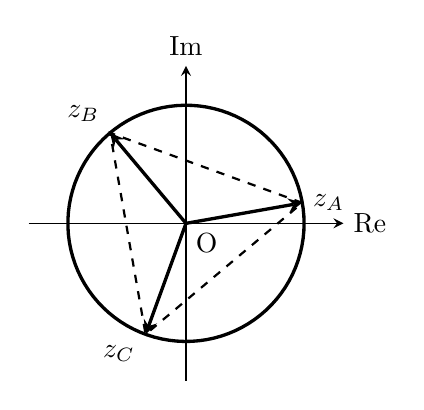
\begin{tikzpicture}
      \draw[->,>=stealth,semithick] (-2,0)--(2,0)node[right]{Re}; %x軸
      \draw[->,>=stealth,semithick] (0,-2)--(0,2)node[above]{Im}; %y軸
      \draw (0,0)node[below right]{O};
      \draw[very thick,samples=100,domain=0:2*pi,variable=\theta] plot(\theta r:1.5);
      \draw[very thick,->,>=stealth] (0,0)--(10:1.5)node[right]{$z_A$};
      \draw[very thick,->,>=stealth] (0,0)--(130:1.5)node[above left]{$z_B$};
      \draw[very thick,->,>=stealth] (0,0)--(250:1.5)node[below left]{$z_C$};
      \draw[thick, dashed] (10:1.5)--(130:1.5)--(250:1.5)--(10:1.5);
    \end{tikzpicture}
  \end{center}
  \caption{単位円による解析}
  \label{fig:circle}
\end{figure}